\section{Grundlagen relationaler Datenbanken}
\label{section:basics}

Die grundlegende Struktur relationaler Datenbanken ist aufgrund der weiten Verbreitung und Anwendung von Tabellenkalkulations-Software einfach zu verstehen. Relationale Datenbanken bestehen aus Tabellen, die in Relation zueinander stehen. Jeder Objekttyp oder auch Entitätstyp wird in einer eigenen Tabelle definiert, wobei die Spalten die Attribute des Objekts darstellen. Die Festlegung der Objekttypen, ihrer Attribute, und Beziehungstypen wird insbesondere für Datenbanken mit >10 Tabellen schnell komplex. Es empfiehlt sich daher eine strukturierte  Konstruktion dieser Tabellen und ihrer Beziehungstypen. 

Der Aufbau einer Datenbankstruktur vom Entwurf bis zu der konkreten Realisierung wird in (\cite{kaufmannSQLNoSQLDatenbanken92023}: 29ff) in drei Schritten beschrieben: 1. Anforderungsanalyse, 2. konzeptionelle Datenmodellierung und 3. Implementierung des Datenbankschemas durch Abbildung auf ein spezifisches Datenbankmodell (in dieser Arbeit: ein Relationenmodell). Diese Schritte werden in diesem Kapitel anhand eines vereinfachten Modells der \glqq Carsharing App\grqq\ beispielhaft beschrieben und im Hauptteil detailliert ausgeführt.

\subsection{Anforderungsanalyse}
Eine gute Anforderungsanalyse sollte die Wünsche und Ziele der Personen berücksichtigen, die mit der Applikation arbeiten oder diese verwenden. Für den späteren Entwurf der Datenbank ist es wichtig, dass die notwendigen Informationen in der Sprache der Anwendenden formuliert werden (\cite{kaufmannSQLNoSQLDatenbanken92023}: 31), und die Abstraktion zu konkreten Datensätzen erst im nächsten Schritt erfolgt. Im Beispiel der \glqq Carsharing Applikation \grqq\ sollten potentielle Kund:innen, die Entwickler:innen, die Buchhaltung sowie mögliche weitere Beteiligte nach den für sie benötigten Informationen befragt werden. Au\ss erdem können Konkurrenzunternehmen analysiert werden, insbesondere wenn es um die Ausgestaltung der Informationen geht, die in Konkurrenz-Applikationen bereits ersichtlich sind. Beispielhaft ergibt sich für die \glqq Carsharing Applikation \grqq\ die in \autoref{fig:Anforderungsanalyse} gezeigte Anforderungsanalyse. Für das Beispiel wurde die Anforderungsanalyse anhand einer realen Applikation nachgezeichnet und ist daher nicht vollständig.

\begin{figure}[htb]
	\centering
	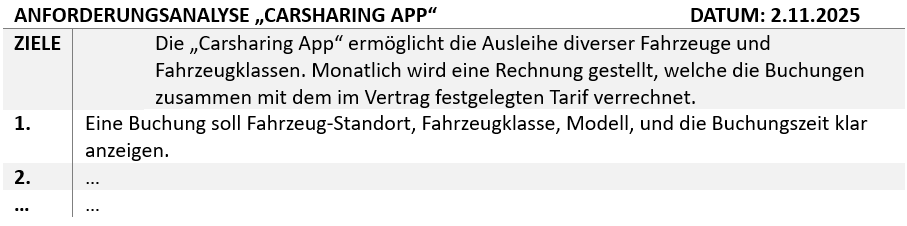
\includegraphics[width=\linewidth]{./pictures/Anforderungsliste}
	\caption{Eine für die theoretische Betrachtung der Datenbankmodellierung verkürzte Anforderungsanalyse der \glqq Carsharing Applikation\grqq.}
	\label{fig:Anforderungsanalyse}
\end{figure}

\subsection{Konzeptionelle Datenmodellierung}
Aus der Anforderungsanalyse wird das \textit{semantische Modell} in Form z.B. eines Entitaeten-Beziehungsmodells (Entity-Relationship-Modell, ERM) erarbeitet (\cite{gehringWirtschaftsinformatik2022}: 18). Ähnlich den Klassen in der objektorientierten Programmierung werden Entitäts-Typen festgelegt und mit bestimmten Eigenschaften (Attributen) definiert und gegenseitige Entitaets-Beziehungstypen abgeleitet. Die Beziehungstypen sind durch Assoziationen mengenmäßig verknüpft, sodass beispielsweise einem Kunden mehrere Rechnungen zugeordnet sein können, eine Rechnung jedoch nicht mehreren Kunden zugeordnet sein kann. Wie in \autoref{fig:ERM-Diagram-Definitionen} dargestellt, wurden für das ERM feste Symbole festgelegt um Entitätstypen (Rechteck), Beziehungstypen (Raute), Assoziationen (Pfeile) und Attribute (Kreise) darzustellen. Für die Darstellung der Assoziationen existieren mehrere Darstellungen, wobei sich diese Arbeit auf die ursprüngliche Chen-Notation (1:1, 1:n, n:1, n:m) beschränkt (\cite{gluchowskiDatenmodellierungDataWarehouseSystemenKonzepte2025}: 36).

\begin{figure}[htb]
	\centering
	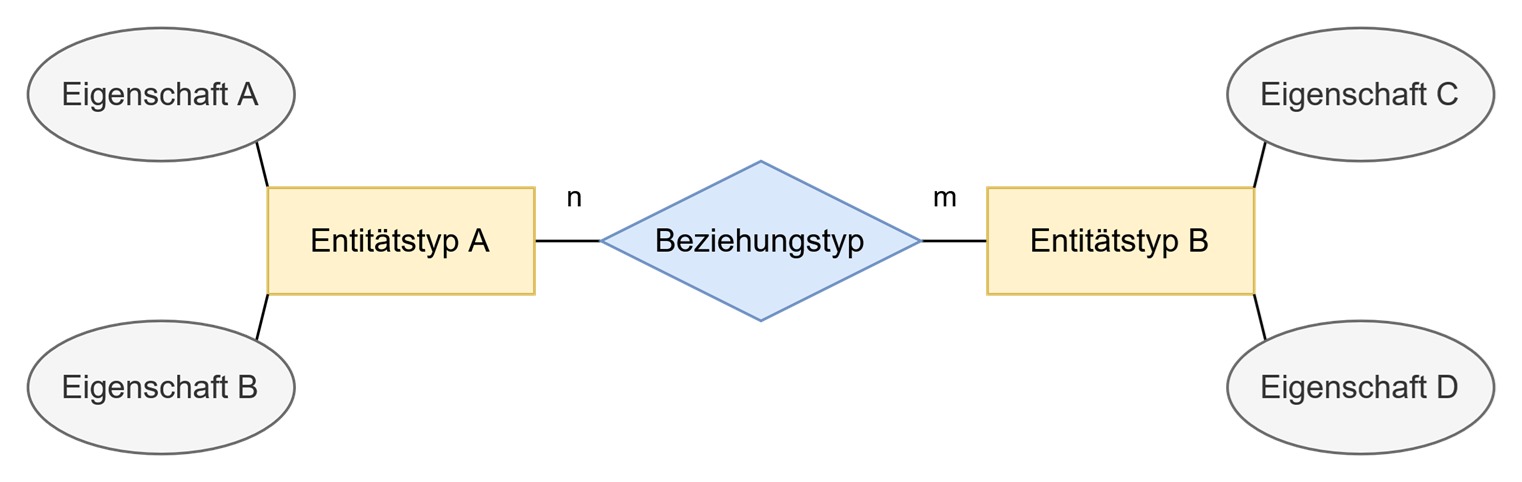
\includegraphics[width=\linewidth]{./pictures/ERM-Diagram-Definitionen}
	\caption{ERM-Darstellung für Entitätstypen (Rechteck), Beziehungstypen (Raute), Assoziationen (Pfeile) und Attribute (Kreise). Die Assoziationen sind in der Chen-Notation 1:1, 1:n, oder n:m dargestellt. Die Farben dienen nur der Übersichtlichkeit.}
	\label{fig:ERM-Diagram-Definitionen}
\end{figure}

Für das Beispiel der \glqq Carsharing Applikation\grqq\ sollen sich für das bessere Verständnis der nachfolgenden Schritte in der Datenmodellierung nur die Entitätstypen Kunde und Fahrzeug-Buchung ergeben. Die ausführliche Darstellung findet sich im Hauptteil dieser Arbeit.

\subsection{Abbildung auf Relationenmodell}
\label{subsec:Abbildung auf Relationenmodell}
Während das bisher betrachtete semantische Modell unabhängig war vom Datenbankmodell wird im logischen Schema ein spezifisches Modell festgelegt. In dieser Arbeit wird das Relationenmodell angewendet, welches Anfang der 1970er Jahre von Edgar Frank Codd begründet wurde. Dieser setzte sich unter anderem mit dem mathematisch-logischen Problem einer redundanzfreien Datenmodellierung auseinander (\cite{kaufmannSQLNoSQLDatenbanken92023}: 14).

In einer Veröffentlichung von 1970 beschrieb Codd (\cite{coddRelationalModelData1970}) bestimmte Regeln für die Erstellung und Optimierung einer Datenstruktur im relationalen Modell, die weiterhin gültig sind. Nach Codd bestehen relationale Datenstrukturen aus Relationen (engl. relations) auf Eigenschaften, die als Tupel (engl. set) definiert sind. Die einzelnen Elemente dieses Tupels nennt Codd auch Domänen (engl. domains) (\cite{coddRelationalModelData1970}: 379). Hieraus leitet sich direkt eine Zusammengehörigkeit dieser Eigenschaften zu einer Relation heraus, die man sich graphisch als Baumstruktur oder auch Tabelle vorstellen kann. Die Baumstruktur (vgl. Darstellung in \cite{coddRelationalModelData1970}: 379) bietet den Vorteil, dass \glqq non-simple domains\grqq\ übersichtlicher dargestellt werden können, während in Tabellen diese \glqq non-simple domains\grqq\ in weitere Relationen-Tabellen ausgegliedert und deren ursprüngliche Beziehungen durch Primär- und Fremdschlüssel festgehalten werden (\cite{kaufmannSQLNoSQLDatenbanken92023}: 41ff). Aufgrund der Komplexität der Datenmodellierung ist es sinnvoll, die verschiedenen Darstellungsformen und deren Einsatzgebiete zu verstehen.

Tabelle \ref{table:Buchung} zeigt die Relation \textit{Buchung} als vereinfachte Form für unser Beispiel einer \glqq Carsharing Applikation\grqq (im Hauptteil weiter ausgeführt). Das Tupel, das die Eigenschaften festlegt lautet (ID, Buchungszeit, Fahrzeug, Standort).  Zeilenweise werden darunter Datensätze dargestellt, wobei die Zeilenreihenfolge (im Gegensatz zur Reihenfolge der Spalten) egal ist. In jeder Relation wird ein Primärschlüssel festgelegt, der jeden Eintrag eindeutig festlegt und nicht doppelt vorkommen kann. Wichtig ist nur die Eindeutigkeit, daher ist auch eine Kombination von Attributen möglich, die einzeln nicht eindeutig sind, aber in Kombination nur ein Mal auftreten. Hierbei ist zu beachten, dass diese Kombination auch in einer wachsenden Tabelle immer noch eindeutig sein muss, weswegen es oft einfacher sein kann eine eindeutige ID für neue Einträge zu vergeben. Im Beispiel wird eine solche ID als Primärschlüssel verwendet.

\begin{table}[htb]
	
	\centering
	\caption{Buchung}\label{table:Buchung}
	\begin{tabular}{llllllll} \toprule
		ID & Buchungszeit & Fahrzeug & Standort \\ 
		\midrule
		000 & 14.10.25, 15:00-17:00 & Touran, M & Amselweg 15, 8888 Musterstadt \\
		003 & 11.03.22, 08:00-11:00 & Multivan, L & Spatzengasse 26, 7777 Musterhausen \\
		001 & 25.09.25, 11:00-17:00 & Punto, S & Möweninsel 13, 7777 Musterhausen \\
		004 & 25.09.25, 11:00-17:00 & Twingo, S & Möweninsel 13, 7707 Musterhausen \\
		\bottomrule
	\end{tabular}
\end{table}


Die redundanzarme Datenmodellierung erfolgt in mehreren Schritten die Codd als \textit{Normalisierung} bezeichnete: "There is, in fact, a very simple elimination procedure, which we shall call normalization\  (\cite{coddRelationalModelData1970}: 381)". Nachfolgend sollen die drei Formen der Normalisierung auf die Tabelle \ref{table:Buchung} beispielhaft angewendet werden.

\paragraph{1. Normalform}
Eine Relation befindet sich in der 1. Normalform, wenn alle Attribute atomare, d.h. nicht weiter unterteilbare Attributausprägungen aufweisen (\cite{gehringWirtschaftsinformatik2022}: 798). In Tabelle \ref{table:Buchung} zeigt sich, dass das Attribut Fahrzeug neben dem Fahrzeugnamen auch die Fahrzeugklasse enthält, wobei unterschiedliche Fahrzeugnamen der gleichen Klasse zugeordnet sind. Zudem findet sich eine Doppelung der Einzel-Einträge von \glqq Adresse, Hausnummer, PLZ, Stadt\grqq\ bei der Kategorie Standort. Durch Aufteilung in eigene Attribute ergibt sich daher die 1. Normalform in Tabelle \ref{table:1NF:Buchung}.

\begin{table}[!ht]
	
	\centering
	\caption{Buchung (1.Normalform)}\label{table:1NF:Buchung}
	\begin{tabular}{llllllll} \toprule
		ID 	& Buchungszeit & Fahrzeug & Typ & Stra\ss e & Nr & PLZ & Stadt \\ 
		\midrule
		000 & 14.10.25 15:00-17:00 & Touran & M & Amselweg & 15 & 8888 & Musterstadt \\
		003 & 11.03.22 08:00-11:00 & Multivan & L & Spatzengasse & 26 & 7777 & Musterhausen \\
		001 & 25.09.25 11:00-17:00 & Punto & S & Möweninsel & 13 & 7777 & Musterhausen \\
		004 & 25.09.25 11:00-17:00 & Twingo & S & Möweninsel & 13 & 7707 & Musterhausen \\
		\bottomrule
	\end{tabular}
\end{table}

\paragraph{2. Normalform}
Ausgehend von einer Relation, die sich bereits in der 1. Normalform befindet, ergibt sich die 2. Normalform wenn jedes Nichtschlüsselattribut vom Identifikationsschlüssel voll-funktional abhängig ist. (\cite{gehringWirtschaftsinformatik2022}: 799). In der Relation Buchung (\autoref{table:1NF:Buchung}) ist die Buchungs-ID der Primärschlüssel und das Attribut Buchungszeit voll-funktional von diesem abhängig. Die weiteren Attribute sind jedoch nur teil-funktional von der Buchungs-ID abhängig. Fahrzeug und Typ sind stattdessen voll-funktional abhängig von einem bestimmten Fahrzeug (\autoref{table:2NF:Fahrzeug}) und die Stra\ss e, Nr, PLZ und Stadt sind nur voll-funktional abhängig von einem bestimmten Standort des Fahrzeugs (siehe \autoref{table:2NF:Standort}). Die Auflösung dieser teil-funktionalen Abhängigkeiten erfolgt durch die Aufspaltung in separate Relationen (Tabellen). Die Verbindung der Relationen wird durch Fremdschlüssel definiert, die beispielsweise in der Relation Buchung (\autoref{table:2NF:Buchung}) das Fahrzeug und den Standort des Fahrzeugs festhalten. Zur Kennzeichnung werden die Primärschlüssel und Fremdschlüssel unterstrichen. Fremdschlüssel wurden in dieser Arbeit außerdem kursiv geschrieben.

\begin{table}[!ht]
	\centering
	\caption{Buchung (2. Normalform)}\label{table:2NF:Buchung}
	\begin{tabular}{llllllll} \toprule
		\underline{Buchungs-ID} & Buchungszeit & \textit{\underline{Fahrzeug}} & \textit{\underline{Standort}}	 \\ 
		\midrule
		000&  14.10.25 15:00-17:00  & R-AA-123 & 000 \\
		003&   11.03.22 08:00-11:00 & M-XY-321 & 001  \\
		001&   25.09.25 11:00-17:00 & M-QE-355 & 002  \\
		004&   25.09.25 11:00-17:00 & M-SR-411 & 003  \\
		\bottomrule
	\end{tabular}
%\end{table}

%\begin{table}
	\parbox{.35\linewidth}{
	\centering
	\caption{Fahrzeug (2. Normalform)}\label{table:2NF:Fahrzeug}
	\begin{tabular}{lll} \toprule
		\underline{Fahrzeug} 	& Modell & Typ \\ 
		\midrule
		R-AA-123 & Touran & M    \\
		M-XY-321 & Multivan & L  \\
		M-QE-355 & Punto & S     \\
		M-SR-411 & Twingo & S    \\
		\bottomrule
	\end{tabular}
	}
	\hfill
	\parbox{.62\linewidth}{
	\centering
	\caption{Standort (2. Normalform)}\label{table:2NF:Standort}
	\begin{tabular}{lllll} \toprule
	\underline{Standort} 	& Stra\ss e & Nr & PLZ & Stadt \\ 
	\midrule
	000 & Amselweg & 15 & 8888 & Musterstadt \\
	001 & Spatzengasse & 26 & 7777 & Musterhausen \\
	002 & Möweninsel & 13 & 7777 & Musterhausen \\
	003 & Möweninsel & 13 & 7707 & Musterhausen \\
	\bottomrule
\end{tabular}
	}
\end{table}

\paragraph{3. Normalform}
Ausgehend von einer Relation die sich bereits in der 2. Normalform befindet, ergibt sich die 3. Normalform wenn kein Attribut transitiv vom Primärschlüsselattribut abhängt. In der Tabelle \ref{table:2NF:Standort} ist die Stadt primär abhängig von der PLZ. Eine Stadt kann mehrere PLZ besitzen, jedoch ist jede PLZ eindeutig einer Stadt zugehörig. Die Stadt ist daher nur transitiv vom Primärschlüssel des Standorts abhängig. Eine Auflösung dieser inneren Redundanz kann durch die Aufspaltung von \autoref{table:2NF:Standort} in eine weitere Relation Ortsnamen (\autoref{table:3NF:Ortsname}) erfolgen, in welcher die PLZ mit den Ortsnamen verknüpft sind. Die Relation zur \autoref{table:3NF:Ortsname} wird in dieser durch den Fremdschlüssel PLZ mit \autoref{table:3NF:Standort} verknüpft.

\begin{table}[ht]
	\parbox{.5\linewidth}{
	\centering
	\caption{Standort (3. Normalform)}
	\label{table:3NF:Standort}
	\begin{tabular}{lllll} \toprule
		\underline{Standort} 	& Stra\ss e & Nr & \textit{\underline{PLZ}}\\ 
		\midrule
		000 & Amselweg & 15 & 8888 \\
		001 & Spatzengasse & 26 & 7777 \\
		002 & Möweninsel & 13 & 7777 \\
		003 & Möweninsel & 13 & 7707 \\
		\bottomrule
	\end{tabular}
	}
	\hfill
	\parbox{.5\linewidth}{
		\centering
		\caption{Ortsname (3. Normalform)}
		\label{table:3NF:Ortsname}
		\begin{tabular}{ll} \toprule
			\underline{PLZ} 	& Stadt \\ 
			\midrule
			8888 & Musterstadt \\
			7777 & Musterhausen \\
			7777 & Musterhausen \\
			7707 & Musterhausen \\
			\bottomrule
		\end{tabular}
	}
\end{table}

Insbesondere der letzte Normalisierungsschritt in dem Beispiel zeigt, dass es nicht immer sinnvoll ist, die Regeln der Normalisierung beim Datenbankentwurf strikt zu befolgen. Die Ausgliederung des Ortsnamens erzeugt eine zusätzliche Tabelle die über einen zusätzlichen Fremdschlüssel gespeichert und bei einer Abfrage zusätzlich abgerufen werden muss. Allgemein bietet die Codd'sche Normalisierung jedoch eine gute Grundlage, um ausgehend von einer möglichst redundanzfreien Struktur nur die Redundanzen aufzulösen, welche die anfänglich genannten Ziele einer geringen Redundanz, guten Bedienbarkeit, flexiblen Erweiterbarkeit, hohen Performance, der Konsistenz und Integrität bestmöglich erfüllen.

Ausgehend von dieser theoretischen Betrachtung einer Datenbankmodellierung wird im nächsten Kapitel die vollständige Datenbank einer potentiellen \glqq Carsharing App\grqq\ entworfen und beispielhaft gezeigt, wie die Daten in einem Datenbankverwaltungssystem mittels der Datenbanksprache SQL abgerufen und bearbeitet werden können.











